
%% bare_jrnl.tex
%% V1.1
%% 2002/08/13
%% by Michael Shell
%% mshell@ece.gatech.edu
%%
%% NOTE: This text file uses MS Windows line feed conventions. When (human)
%% reading this file on other platforms, you may have to use a text
%% editor that can handle lines terminated by the MS Windows line feed
%% characters (0x0D 0x0A).
%%
%% This is a skeleton file demonstrating the use of IEEEtran.cls
%% (requires IEEEtran.cls version 1.6 or later) with an IEEE journal paper.
%%
%% Support sites:
%% http://www.ieee.org
%% and/or
%% http://www.ctan.org/tex-archive/macros/latex/contrib/supported/IEEEtran/
%%
%% This code is offered as-is - no warranty - user assumes all risk.
%% Free to use, distribute and modify.

% *** Authors should verify (and, if needed, correct) their LaTeX system  ***
% *** with the testflow diagnostic prior to trusting their LaTeX platform ***
% *** with production work. IEEE's font choices can trigger bugs that do  ***
% *** not appear when using other class files.                            ***
% Testflow can be obtained at:
% http://www.ctan.org/tex-archive/macros/latex/contrib/supported/IEEEtran/testflow


% Note that the a4paper option is mainly intended so that authors in
% countries using A4 can easily print to A4 and see how their papers will
% look in print. Authors are encouraged to use U.S. letter paper when
% submitting to IEEE. Use the testflow package mentioned above to verify
% correct handling of both paper sizes by the author's LaTeX system.
%
% Also note that the "draftcls", not "draft", option should be used if
% it is desired that the figures are to be displayed in draft mode.

% *************************************************************************
% You can now use this template both for submitting to peer review and,
% if your paper is accepted, for sending in final publication materials.
% To change from peer review format (single column, double-spaced) to
% final publication format (double column, single-spaced), just move the
% comment-line sign (%) from one \documentclass line to the other.
% The first is for peer review format(single column), the second is for final publication(double column).

%\documentclass[12pt,journal,draftcls,letterpaper,onecolumn]{IEEEtran}
%\documentclass[9.5pt,journal,final,finalsubmission,twocolumn]{IEEEtran}
\documentclass[10pt,journal,letterpaper,compsoc,peerreview]{IEEEtran}
\usepackage{pifont}
\usepackage{multirow}
\usepackage{comment}
\usepackage{subfigure}
\usepackage{color}
\usepackage{epsfig}
\usepackage{times}
\usepackage{url}
\usepackage[nocompress]{cite}
% *************************************************************************


% If the IEEEtran.cls has not been installed into the LaTeX system files,
% manually specify the path to it:
% \documentclass[journal,draftcls,onecolumn]{../sty/IEEEtran}


% some very useful LaTeX packages include:

%\usepackage{cite}      % Written by Donald Arseneau
                        % V1.6 and later of IEEEtran pre-defines the format
                        % of the cite.sty package~\cite{} output to follow
                        % that of IEEE. Loading the cite package will
                        % result in citation numbers being automatically
                        % sorted and properly "ranged". i.e.,
                        % [1], [9], [2], [7], [5], [6]
                        % (without using cite.sty)
                        % will become:
                        % [1], [2], [5]--[7], [9] (using cite.sty)
                        % cite.sty's~\cite will automatically add leading
                        % space, if needed. Use cite.sty's noadjust option
                        % (cite.sty V3.8 and later) if you want to turn this
                        % off. cite.sty is already installed on most LaTeX
                        % systems. The latest version can be obtained at:
                        % http://www.ctan.org/tex-archive/macros/latex/contrib/supported/cite/

%\usepackage{graphicx}  % Written by David Carlisle and Sebastian Rahtz
                        % Required if you want graphics, photos, etc.
                        % graphicx.sty is already installed on most LaTeX
                        % systems. The latest version and documentation can
                        % be obtained at:
                        % http://www.ctan.org/tex-archive/macros/latex/required/graphics/
                        % Another good source of documentation is "Using
                        % Imported Graphics in LaTeX2e" by Keith Reckdahl
                        % which can be found as esplatex.ps and epslatex.pdf
                        % at: http://www.ctan.org/tex-archive/info/

%\usepackage{psfrag}    % Written by Craig Barratt, Michael C. Grant,
                        % and David Carlisle
                        % This package allows you to substitute LaTeX
                        % commands for text in imported EPS graphic files.
                        % In this way, LaTeX symbols can be placed into
                        % graphics that have been generated by other
                        % applications. You must use latex->dvips->ps2pdf
                        % workflow (not direct pdf output from pdflatex) if
                        % you wish to use this capability because it works
                        % via some PostScript tricks. Alternatively, the
                        % graphics could be processed as separate files via
                        % psfrag and dvips, then converted to PDF for
                        % inclusion in the main file which uses pdflatex.
                        % Docs are in "The PSfrag System" by Michael C. Grant
                        % and David Carlisle. There is also some information
                        % about using psfrag in "Using Imported Graphics in
                        % LaTeX2e" by Keith Reckdahl which documents the
                        % graphicx package (see above). The psfrag package
                        % and documentation can be obtained at:
                        % http://www.ctan.org/tex-archive/macros/latex/contrib/supported/psfrag/

%\usepackage{subfigure} % Written by Steven Douglas Cochran
                        % This package makes it easy to put subfigures
                        % in your figures. i.e. "figure 1a and 1b"
                        % Docs are in "Using Imported Graphics in LaTeX2e"
                        % by Keith Reckdahl which also documents the graphicx
                        % package (see above). subfigure.sty is already
                        % installed on most LaTeX systems. The latest version
                        % and documentation can be obtained at:
                        % http://www.ctan.org/tex-archive/macros/latex/contrib/supported/subfigure/

%\usepackage{url}       % Written by Donald Arseneau
                        % Provides better support for handling and breaking
                        % URLs. url.sty is already installed on most LaTeX
                        % systems. The latest version can be obtained at:
                        % http://www.ctan.org/tex-archive/macros/latex/contrib/other/misc/
                        % Read the url.sty source comments for usage information.

%\usepackage{stfloats}  % Written by Sigitas Tolusis
                        % Gives LaTeX2e the ability to do double column
                        % floats at the bottom of the page as well as the top.
                        % (e.g., "\begin{figure*}[!b]" is not normally
                        % possible in LaTeX2e). This is an invasive package
                        % which rewrites many portions of the LaTeX2e output
                        % routines. It may not work with other packages that
                        % modify the LaTeX2e output routine and/or with other
                        % versions of LaTeX. The latest version and
                        % documentation can be obtained at:
                        % http://www.ctan.org/tex-archive/macros/latex/contrib/supported/sttools/
                        % Documentation is contained in the stfloats.sty
                        % comments as well as in the presfull.pdf file.
                        % Do not use the stfloats baselinefloat ability as
                        % IEEE does not allow \baselineskip to stretch.
                        % Authors submitting work to the IEEE should note
                        % that IEEE rarely uses double column equations and
                        % that authors should try to avoid such use.
                        % Do not be tempted to use the cuted.sty or
                        % midfloat.sty package (by the same author) as IEEE
                        % does not format its papers in such ways.

\usepackage{amsmath}   % From the American Mathematical Society
                        % A popular package that provides many helpful commands
                        % for dealing with mathematics. Note that the AMSmath
                        % package sets \interdisplaylinepenalty to 10000 thus
                        % preventing page breaks from occurring within multiline
                        % equations. Use:
%\interdisplaylinepenalty=2500
                        % after loading amsmath to restore such page breaks
                        % as IEEEtran.cls normally does. amsmath.sty is already
                        % installed on most LaTeX systems. The latest version
                        % and documentation can be obtained at:
                        % http://www.ctan.org/tex-archive/macros/latex/required/amslatex/math/



% Other popular packages for formatting tables and equations include:

% Frank Mittelbach's and David Carlisle's array.sty which improves the
% LaTeX2e array and tabular environments to provide better appearances and
% additional user controls. Array.sty is already installed on most systems.
% The latest version and documentation can be obtained at:
% http://www.ctan.org/tex-archive/macros/latex/required/tools/

% Mark Wooding's extremely powerful MDW tools, especially mdwmath.sty and
% mdwtab.sty which are used to format equations and tables, respectively.
% The MDWtools set is already installed on most LaTeX systems. The lastest
% version and documentation is available at:
% http://www.ctan.org/tex-archive/macros/latex/contrib/supported/mdwtools/

% V1.6 of IEEEtran contains the IEEEeqnarray family of commands that can
% be used to generate multiline equations as well as matrices, tables, etc.


% Also of notable interest:

% Scott Pakin's eqparbox package for creating (automatically sized) equal
% width boxes. Available:
% http://www.ctan.org/tex-archive/macros/latex/contrib/supported/eqparbox/




% *** Do not adjust lengths that control margins, column widths, etc. ***
% *** Do not use packages that alter fonts (such as pslatex).         ***
% There should be no need to do such things with IEEEtran.cls V1.6 and later.


% correct bad hyphenation here
%\hyphenation{op-tical net-works semi-conduc-tor}


\begin{document}
%
% paper title
\title{A novel heuristic for local multiple alignment of interspersed DNA repeats}
%
%
% author names and IEEE memberships
% note positions of commas and nonbreaking spaces ( ~ ) LaTeX will not break
% a structure at a ~ so this keeps an author's name from being broken across
% two lines.
% use \thanks{} to gain access to the first footnote area
% a separate \thanks must be used for each paragraph as LaTeX2e's \thanks
% was not built to handle multiple paragraphs

\author{Todd~J.~Treangen,
        Aaron~E.~Darling,
        Guillaume~Achaz,
        Mark~A.~Ragan,
        and~Xavier~Messeguer% <-this % stops a space
        }

\IEEEcompsocitemizethanks{
\IEEEcompsocthanksitem T.J. Treangen is with the Microbial Evolutionary Genomics group, Institut Pasteur, Paris, France \protect\\ and the UPMC Univ Paris 06, Atelier de Bioinformatique, Paris, France
\IEEEcompsocthanksitem A.E. Darling is with the Institute for Molecular Bioscience, The University of Queensland, Brisbane, Australia
\IEEEcompsocthanksitem G. Achaz is with the UPMC Univ Paris 06, CNRS, MNHN, IRD, UMR 7138, Paris, France  \protect\\ and the UPMC Univ Paris 06, Atelier de Bioinformatique, Paris, France
\IEEEcompsocthanksitem M. Ragan is with the Institute for Molecular Bioscience, The University of Queensland, Brisbane, Australia
\IEEEcompsocthanksitem X. Messeguer is with the Algorithms and Genetics Group,Dept. of Computer Science, Technical University of Catalonia, Barcelona, Spain
\IEEEcompsocthanksitem T.J. Treangen and A.E. Darling contributed equally to this work.}


% \author{....lastname \thanks{...} \thanks{...} }
%                     ^------------^------------^----Do not want these spaces!
%
% a space would be appended to the last name and could cause every name on that
% line to be shifted left slightly. This is one of those "LaTeX things". For
% instance, "A\textbf{} \textbf{}B" will typeset as "A B" not "AB". If you want
% "AB" then you have to do: "A\textbf{}\textbf{}B"
% \thanks is no different in this regard, so shield the last } of each \thanks
% that ends a line with a % and do not let a space in before the next \thanks.
% Spaces after \IEEEmembership other than the last one are OK (and needed) as
% you are supposed to have spaces between the names. For what it is worth,
% this is a minor point as most people would not even notice if the said evil
% space somehow managed to creep in.
%
% The paper headers
%\markboth{Journal of \LaTeX\ Class Files,~Vol.~1, No.~8,~August~2002}{Shell \MakeLowercase{\textit{et al.}}: Bare Demo of IEEEtran.cls for Journals}
% The only time the second header will appear is for the odd numbered pages
% after the title page when using the twoside option.


% If you want to put a publisher's ID mark on the page
% (can leave text blank if you just want to see how the
% text height on the first page will be reduced by IEEE)
%\pubid{0000--0000/00\$00.00~\copyright~2002 IEEE}

% use only for invited papers
\IEEEspecialpapernotice{(Invited Paper)}

% make the title area
\maketitle
%\IEEEdisplaynotcompsoctitleabstractindextext
%\IEEEcompsoctitleabstractindextext{
\begin{abstract}
The identification of homologous DNA is a fundamental building block
of comparative genomic and molecular evolution studies. Pairwise local sequence alignment methods have been the prevailing
technique to identify homologous nucleotides. However, existing
methods that identify and align all homologous nucleotides in one or
more genomes have suffered poor scalability and limited accuracy. We
propose a novel method that couples a gapped extension heuristic with
an efficient filtration method for local multiple
alignment.  During gapped extension, we use the MUSCLE implementation
of progressive multiple alignment with iterative refinement.  The
resulting gapped extensions potentially contain alignments of
unrelated sequence.  We detect and
remove such undesirable alignments using a hidden Markov model to
predict the posterior probability of homology. The HMM
emission frequencies for nucleotide substitutions can be derived from
any strand/species-symmetric nucleotide substitution matrix, and we
have developed a method to adapt an arbitrary substitution matrix
(i.e. HOXD70) to organisms with different G+C content. We evaluate the
performance of our method and previous approaches on a hybrid dataset
of real genomic DNA with simulated interspersed repeats.  Our method
outperforms existing methods in terms of sensitivity,
positive predictive value, and localizing boundaries of homology.   
In addition, we present a statistical test for estimating significance of local
multiple alignments. The
described methods have been implemented in the free, open-source
\texttt{procrastAligner} software, available from: \url{http://alggen.lsi.upc.es/recerca/align/procrastination}
\end{abstract}

\begin{IEEEkeywords}
Sequence alignment, genome comparison, DNA repeats, local alignment
\end{IEEEkeywords}

\IEEEpeerreviewmaketitle
\section{Introduction}
Pairwise local sequence alignment has a long and fruitful history
in computational biology and new approaches continue to be
proposed~\cite{ref-pattern,ref-chaos,ref-yass,ref-kahveciMAP}.
Advanced filtration methods based on spaced-seeds have greatly
improved the sensitivity, specificity, and efficiency of many
local alignment
methods~\cite{ref-zhang04,ref-zhang06,ref-buhler05,ref-xu04,ref-batzoglouNAR}.
Common applications of local alignment can range from orthology
mapping~\cite{ref-orthomcl} to genome assembly~\cite{ref-arachne2}
to information engineering tasks such as data
compression~\cite{ref-ane}. Recent advances in sequence data
acquisition technology~\cite{ref-454, sequencing, hybrid} provide low-cost sequencing
and will continue to fuel the growth of molecular sequence
databases. To cope with advances in data volume, corresponding
advances in computational methods are necessary; thus we present
an efficient method for local multiple alignment of DNA sequence.

Unlike pairwise alignment, local multiple alignment constructs a
single multiple alignment for all occurrences of a motif in one or
more sequences.  The motif occurrences may be identical or have
degeneracy in the form of mismatches and indels.  As such, local
multiple alignments identify the basic repeating units in one or
more sequences and can serve as a basis for downstream analysis
tasks such as multiple genome
alignment~\cite{ref-mauve,ref-mga,ref-mgcat,ref-deweyReview}, global
alignment with repeats~\cite{ref-otherSammethPaper,ref-aba}, or
repeat classification and analysis~\cite{ref-piler}.  Local multiple
alignment differs from traditional pairwise methods for repeat
analysis which either identify repeat families \textit{de
novo}~\cite{ref-reputer} or using a database of known repeat
motifs~\cite{ref-repbase}.

The importance of accurate homology identification to comparative
genomics can not be overestimated~\cite{Kumar07}. To date, pairwise
local sequence alignment
methods such as BLAST~\cite{ref-blastz,ref-ssearch} have been the
prevailing technique to identify homologous nucleotides.  When more
than two copies of a homologous sequence element are present in the
data, pairwise homology detection methods generate a listing of all
possible pairs of homologous elements in the form of pairwise local
alignments.  Apart from the obvious inefficiency of considering all
pairwise homology relationships, a collection of pairwise alignments
is not ideal because they are rarely amenable to comparative genomic
and phylogenetic analysis without further processing into a multiple
alignment.

Local pairwise alignments can be merged to create a multiple alignment
by a variety of
methods~\cite{ref-tba,ref-dialign,ref-related1}. Such methods
commonly assume that pairwise homology relationships are transitive,
such that if nucleotide $a$ is homologous to nucleotide $b$, and $b$
is to $c$, then $a$ must also be homologous to $c$.  Thus, in order to
merge pairwise alignments, such methods must tackle the challenging
problem of resolving inconsistent transitive homology relationships.
Multiple alignment has been demonstrated to be more accurate than
pairwise alignment, especially when dealing with a large number of
divergent sequences~\cite{ref-mlagan,ref-aubergene}.  As the number of
homologous sequences grows, we might expect that the number of
inconsistent relationships in a collection of pairwise alignments
would grow quadratically, whereas a direct multiple alignment method
would provide an increasingly accurate alignment.  Moreover, highly
repetitive regions in the input sequences can cause serious efficiency
problems for pairwise methods, as they create $O(r^{2})$ pairwise
alignments in the presence of a repeat with $r$ copies.  Mammalian Alu
repeats and IS elements in microbes are two common examples of the
overwhelming abundance of repetitive sequence in whole genomes.

Local multiple alignment has the inherent potential to avoid pitfalls
associated with pairwise alignment. Although optimal multiple
alignment under the SP objective function remains
intractable~\cite{ref-wangjiang}, progressive alignment heuristics
offer excellent speed and accuracy~\cite{ref-clustalw,ref-tcoffee}
especially when combined with tree-independent iterative
refinement~\cite{ref-muscle}, or probabilistic consistency
measures~\cite{ref-probcons}. Rather than merging pairwise alignments,
why not exploit years of research into multiple alignment heuristics
by directly constructing a multiple alignment? We thus present a novel
heuristic for directly computing local multiple alignments via gapped
extension of chained seed matches.

\section{A heuristic for gapped extension of local multiple alignments}
Our method for computing local multiple alignments exploits the MUSCLE
multiple alignment algorithm to compute gapped extensions of ungapped
multi-match seeds (see Figure~\ref{fig-main}). Gapped alignments arise
when extending seeds to fully capture surrounding sequence
homology. Our method assumes that a fixed number of nucleotides
flanking a seed match are likely to be homologous and computes a
global multiple alignment on the flanking region.  Our assumption of
flanking homology often proves to be erroneous and results in an
alignment of unrelated sequences.  In the context of \textit{local}
multiple alignment, the fundamental problem with such an approach is
that current methods for progressive alignment with iterative
refinement compute \textit{global} alignments, i.e. they implicitly
assume that input sequences are homologous over their entire length.
To resolve the problem, we employ a hidden Markov model which detects
unrelated regions embedded in the global multiple alignment.
Unrelated regions are then removed from the alignment and the
local-multiple alignment is trimmed to reflect the updated boundaries
of homology.

Our method, depicted for an example sequence in
Figure~\ref{fig-main}, has seven primary steps: (1) identify
multi-match seeds in the input sequence, (2) chain individual
seeds, (3) multiply align of regions between chained seeds, (4)
gapped extension of seed chains (5) detect unrelated regions
using a hidden Markov model, (6) apply transitive homology
relationships and removal of any unrelated sequence from
the final local multiple alignment, and (7) statistical test for rejecting
insignificant local alignments.  Steps 2-8 are applied
repeatedly to seeds identified in step 1 to produce local multiple
alignments of all homologous nucleotides in the input sequence.

\begin{figure}[t!]
\begin{center}
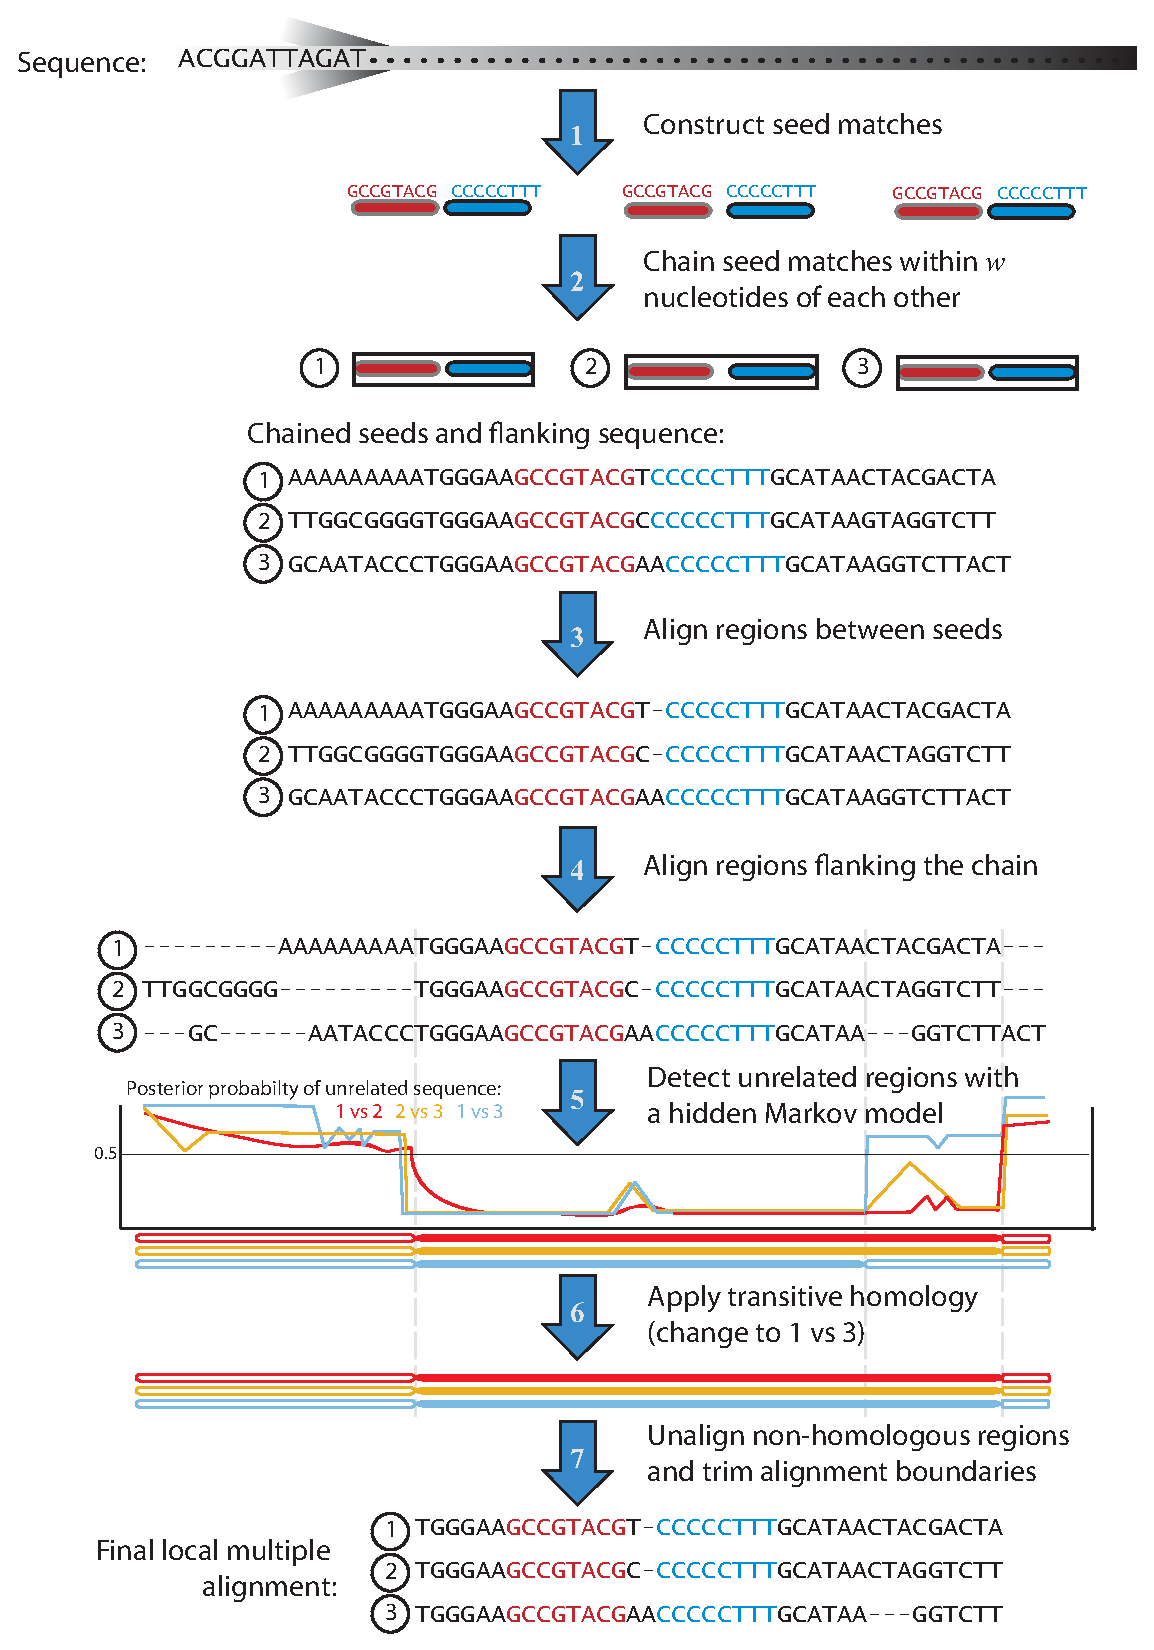
\epsfig{file=./fig/extension.eps,width=3.5in}
%\subfigure[Visual representation of our algorithm]{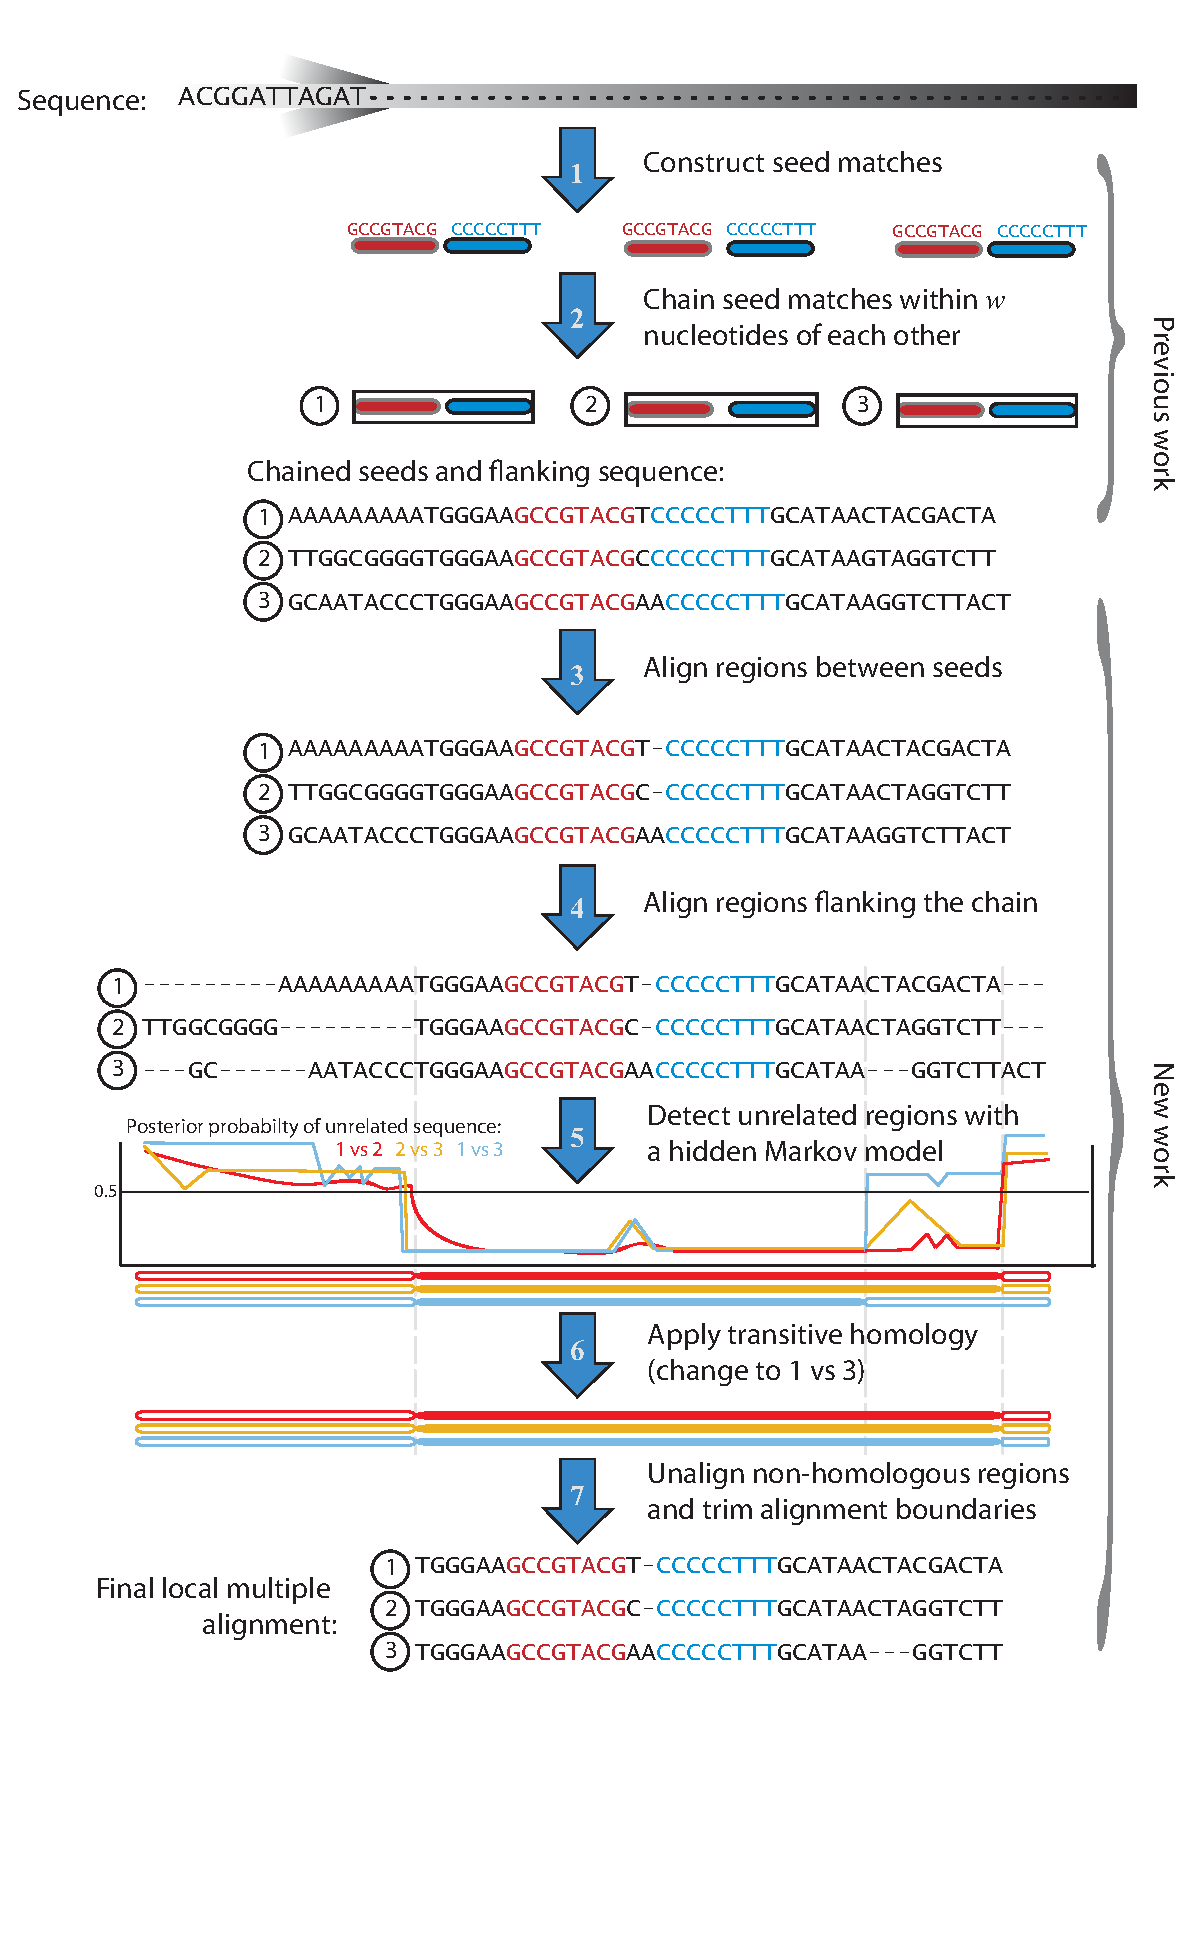
\epsfig{file=./figures/extension.eps,width=3.0in}}
%\subfigure[Flowchart of the algorithmic process ]{ 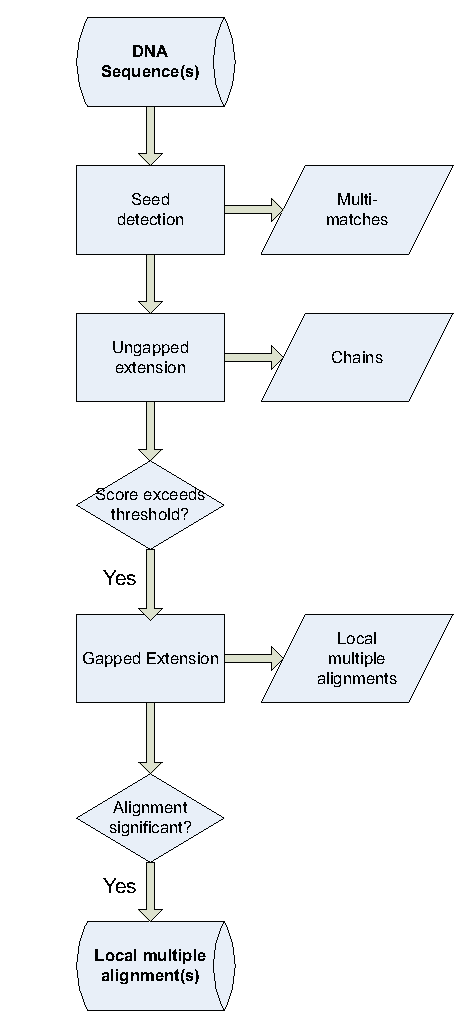
\epsfig{file=./figures/flowchart.eps,width=1.7in}}
\end{center}
%\vspace{-1.6cm}
\caption[Overview of our method for local multiple alignment]%
{\scriptsize Overview of the method, starting with an input sequence and ending
with a set of local multiple alignments. First we (1) detect
multi-matches in the input sequence(s) using palindromic spaced seeds,
then we perform (2) chaining and extension of all multi-matches within
$w$ nt of each other.  In the present example, one chain exists and
contains two matches each with three match components labeled 1, 2,
and 3.  We then perform gapped alignment of the region between chained
matches (3).  In step (4), we perform a gapped extension by computing
a global multiple alignment on the regions to the left and right of
each chain component.  The resulting alignment may contain unrelated
sequence, so in step (5) we apply a hidden Markov model to detect
poorly aligned regions indicative of unrelated sequence and then
compute transitive homology relationships to ensure a consistent
alignment and aid detection of divergent homologous sequences.
In step (6) we unalign regions found to be non-homologous, and
in step (7) we perform a statistic test to reject insignificant
local multiple alignments. If we find after step (2) that the alignment boundaries have been
extended, we return to step (4) for another round of chaining.}
\label{fig-main}
\end{figure}

\subsection{Chaining multi-match seeds from the input sequence}
Given a sequence $\mathcal{S}=s_1, s_2,\dots, s_N$ of length $N$
defined over an alphabet $\{A,C,G,T\}$, our method identifies
local multiple alignments on homologous subsequences of
$\mathcal{S}$. Our method first extracts candidate ungapped
alignments, or multi-matches, among subsequences in $\mathcal{S}$,
and we denote the set of all such matches as $\mathbf{M}$. To extract multi-matches from the input
sequence, we utilize a palindromic spaced seed pattern~\cite{ref-zhang}, which is
analyzed at each position in the input sequence.
Palindromic spaced seeds offer good efficiency and
reasonable sensitivity on a variety of input
sequences~\cite{ref-procrast}.  We refer the number of matching regions
in $\mathcal{S}$ by a given match $M_i \in \mathbf{M}$ as the
\textit{multiplicity} of $M_i$, denoted as $|M_i|$. We refer to each
matching region of $M_i$ as a \textit{component} of $M_i$. Our
algorithm has an important limitation on the matches in $\mathbf{M}$:
no two matches $M_i$ and $M_j$ may have the same left-end coordinate,
except for the identity case when $i=j$.  This constraint has been
referred to by others as \textit{consistency} and
\textit{transitivity}~\cite{ref-transitivity} of matches.

Once a list of multi-matches has been generated, we employ an
efficient chaining and filtration algorithm to identify overlapping
and nested chains of multi-matches~\cite{ref-procrast}. In order to
process each region of sequence $\mathcal{O}(1)$ times, matches
are prioritized for chaining in order of decreasing multiplicity.  The
method chains multi-match seeds of the same multiplicity $|M_i|$
occurring within $w$ characters of each other, thus gaps of up to size
$w$ are tolerated.  When a multi-match can
no longer be chained without including a gap larger than $w$
characters, neighboring \textit{subset} matches within $w$ characters
are identified. Each neighboring subset match is then \textit{linked}
to the chained match. We refer to the chained match as a
\textit{superset} match. Rather than immediately extend the subset
match(es), we \textit{procrastinate} and extend the subset match later
when it has the highest multiplicity of any match waiting to be
extended. When chaining a match with a linked superset, we immediately
include the entire region covered by the linked superset match and
thus eliminate the need to re-examine sequence already covered by a
previously chained match.


\begin{comment}
\subsection{Data structures}
Our chaining algorithm begins with an initialization phase that creates three
data structures. The first data structure is a set of \textit{Match
Records} for each match $M \in \mathbf{M}$.  The \textit{Match
Record} stores $M$, a unique identifier for $M$, and two items which
will be described later in Section~\ref{ssec:extend}: a set of
linked match records, and a \textit{subsuming match pointer}. The
linked match records are further subdivided into four classes: a
left and right \textit{superset link}, and left and right
\textit{subset links}.  The \textit{subsuming match pointer} is
initially set to a \textit{NULL} value. Figure~\ref{fig:proc} shows
a schematic of the match record.

We refer to the second data structure as a \textit{Match Position
Lookup Table}, or $\mathbf{P}$. The table has $N$ entries $p_1,
p_2,\dots,p_N$, one per character of $\mathcal{S}$. The entry for
$p_t$ stores the unique identifier of the match $M_i$ and $x$ for
which $M_i.L_x = t$ or the \textit{NULL} identifier if no match has
$t$ as a left-end coordinate. We call the third data structure a
\textit{Match extension procrastination queue}, or simply the
\textit{procrastination queue}. Again, we denote the multiplicity of
a match $M$ by $|M|$. The \textit{procrastination queue} is a binary
heap of matches ordered on $|M|$ with higher values of $|M|$
appearing near the top of the heap. The heap is initially populated
with all $M \in \mathbf{M}$. This queue dictates the order in which
matches will be considered for extension.

\begin{figure}[t!]
\centering 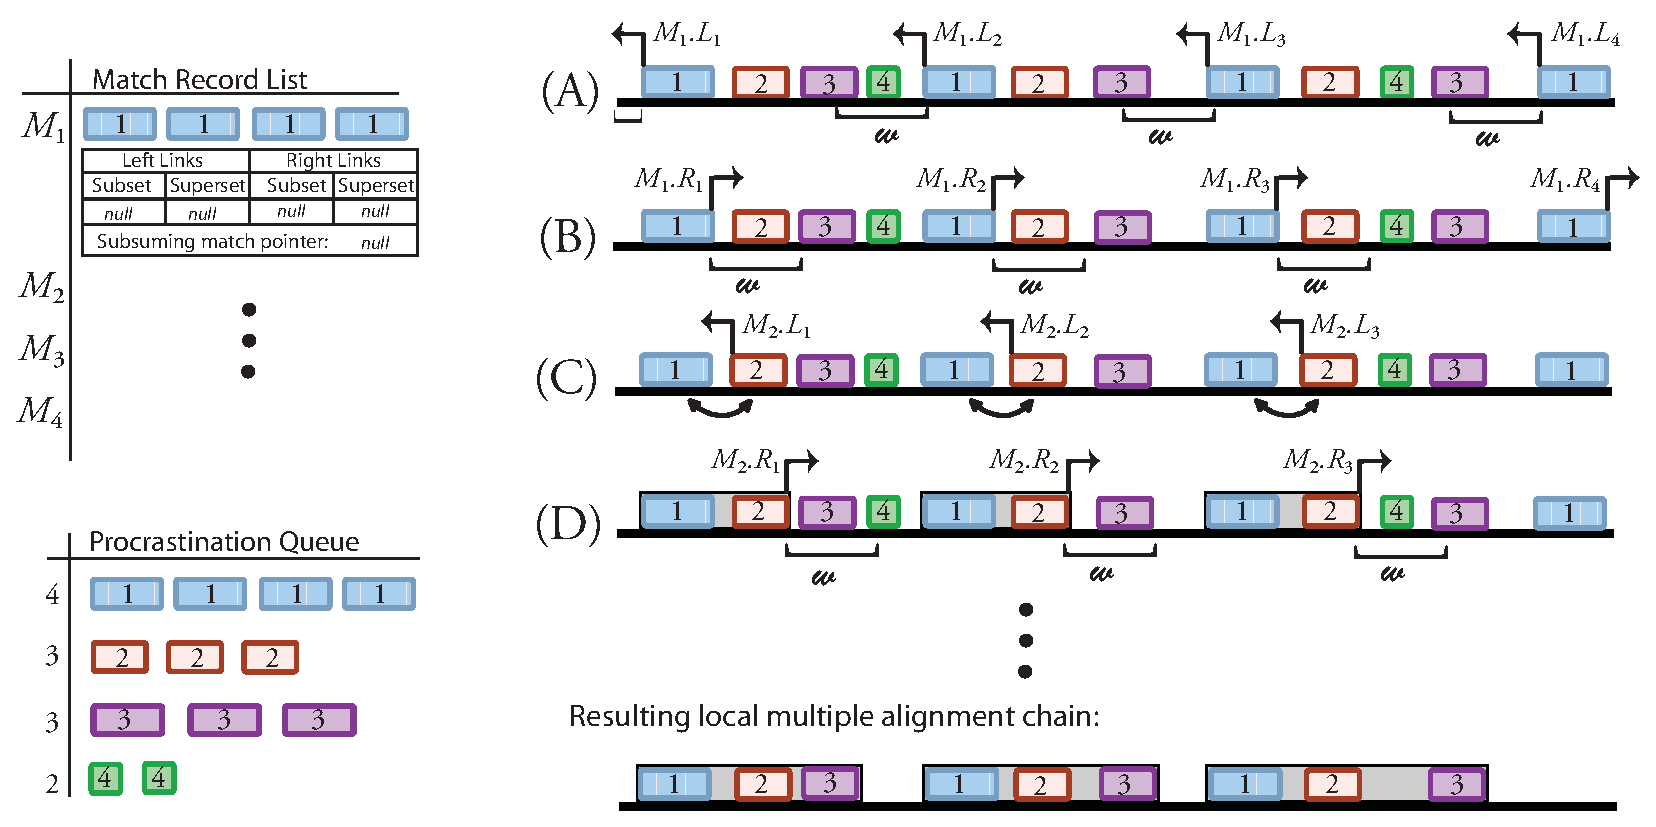
\epsfig{file=fig/proc.pdf,width=3.6in} \caption[The match extension process and associated data
structures]%
{
\looseness=-1 The match extension process and associated data
structures. \textbf{(A)} First we pop the match at the front of the
procrastination queue: $M_{1}$ and begin its leftward extension.
Starting with the leftmost position of $M_{1}$, we use the
\textit{Match Position Lookup Table} to enumerate every match with a
left-end within some distance $w$. Only $M_4.L_1$ is within $w$ of
$M_1$, so it forms a singleton \textit{neighborhood group} which we
discard. \textbf{(B)} $M_1$ has no \textit{neighborhood groups} to
the left, so we begin extending $M_1$ to the right.  We enumerate
all matches within $w$ to the right of $M_1$. $M_2$ lies to the
right of 3 of 4 components of $M_1$ and so is not subsumed, but
instead gets linked as a right-subset of $M_1$. We add a
left-superset link from $M_{2}$ to $M_1$. \textbf{(C)} Once finished
with $M_{1}$ we pop $M_{2}$ from the front of the procrastination
queue and begin leftward extension. We find the left-superset link
from $M_2$ to $M_1$, so we extend the left-end coordinates of
$M_{2}$ to cover $M_{1}$ accordingly. No further leftward extension
of $M_2$ is possible because $M_1$ has no left-subset links.
\textbf{(D)} Beginning rightward extension on $M_{2}$ we construct a
neighborhood list and find a chainable match $M_{3}$, and a subset
$M_{4}$. We extend $M_2$ to include $M_3$ and mark $M_4$ as
inconsistent and hence not extendable. Upon completion of the
chaining process we have generated a list of local multiple
alignments.} \label{fig:proc}
\end{figure}
\end{comment}
\subsection{Gapped extension of high-scoring chains}
Our method computes gapped extensions of the chained multi-match seeds.
After chaining a multi-match $M_i$, we perform gapped alignment on all
collinear regions located between two adjacent components to generate
unextended local multiple alignments. We first evaluate the chain to
decide whether expending computational resources on gapped extension
will be worthwhile. We can optionally require that two or more seeds be present
in the chain and use lower seed weights ($k$), a technique which has
previously been proven
successful~\cite{ref-blastz,ref-gappedblast,ref-blat}.  To perform a
gapped extension in each direction, we use MUSCLE to align dynamically-calculated window
of nucleotides ($l$) to the left and right of the current local
multiple alignment.  Small values of $l$ restrict the alignment search
space, while larger values require more computation but are
potentially more sensitive.  We have empirically determined that
setting $l$ based on multiplicity ($l = 70e^{-0.01*|M_{i}|}$) offers a
good tradeoff between speed and sensitivity.  The resulting extension
window is small for high multiplicity chains,
keeping the alignment search space tractable.
%\begin{equation}
% \max(w, \sqrt{(\max(150^{2}-(2*|M_{i}|)^{2},0)}));
%\end{equation}

\subsection{Identifying unrelated regions}
\begin{figure*}[t!]
\centering 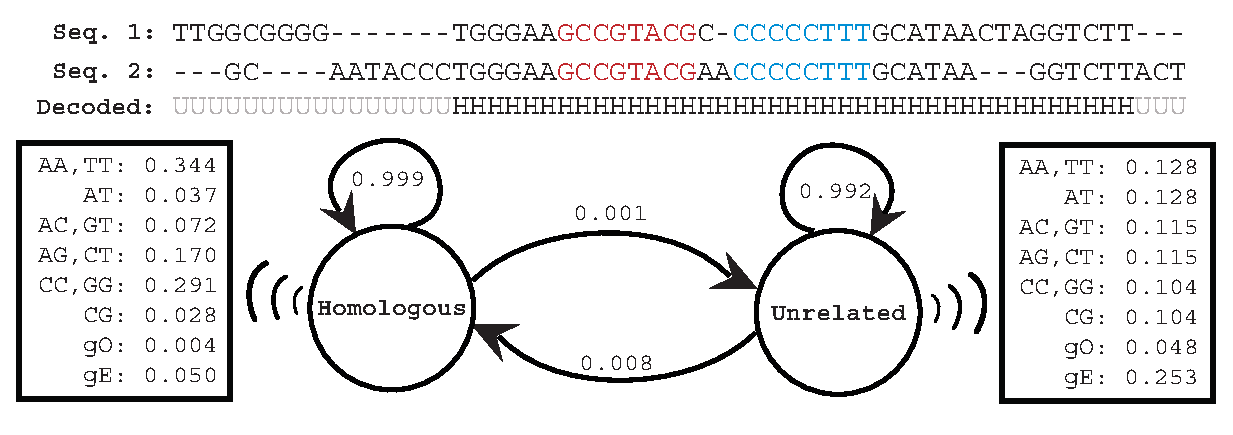
\epsfig{file=./fig/hmm.eps,width=6.8in}
\caption[Hidden Markov model used to detect pairwise alignments of unrelated
sequence]%
{\textbf{Hidden Markov model used to detect pairwise alignments of unrelated
sequence.} The HMM has states which model alignment columns containing
homologous and unrelated sequence. Emission probabilities are extracted from the HOXD70 substitution matrix and correspond to alignment
columns, for example \texttt{AA} indicates A aligned to A.  gO
indicates gap-open and gE gap extend. Alignment columns are treated as
strand-symmetric, so that AC also indicates CA and the reverse
complements TG and GT.  The emission probabilities are adjusted to the G+C content of the input genome
as described in the test.  The values shown here correspond to a 47.5\% G+C genome.}
\label{fig-hmm}
\end{figure*}
The MUSCLE alignment software dutifully reports the highest scoring
global multiple alignment of input sequences, regardless of whether
they are related by common ancestry. As a consequence of the gapped
extension process, it is likely that our method forcibly aligns unrelated
sequence. We have configured a hidden Markov model (Figure
~\ref{fig-hmm}) to detect alignments of unrelated sequence. The HMM
consists of two hidden states, Homologous and Unrelated. The
observable states are the pairwise alignment columns, which are all
possible pairs in $\texttt{{\{A,G,C,T,-\}}}$ with strand and species
symmetry, i.e. \texttt{AG=GA=TC=CT}. The emission probabilities for
each possible pair of aligned nucleotides were extracted from the HOXD70
substitution matrix presented by Chiaromonte \textit{et al.}~\cite{hoxd}.

The resulting emission
probabilities for the Homologous and Unrelated states are given
in Figure~\ref{fig-hmm}. HMM probabilities can be derived using any strand/species-symmetric nucleotide substitution matrix,
but any particular matrix makes specific assumptions about divergence time, mutation pressures,
and sequence composition of the aligned sequences.
Genomes can range in G+C content from 30-75\%, and at the extremes,
a substitution matrix derived on 47.5\% G+C sequence (such as HOXD70) does not
perform well. Previously it has been shown that adapting substitution matrices to the composition
of the organisms under comparison can improve sequence alignment accuracy~\cite{ref-rev3b}.  We have thus developed a method to adapt HMM emission
probabilities derived from an arbitrary substitution matrix
to organisms with different G+C content.

\section{Extracting emission frequencies from the HOXD70 substitution matrix}
We solved for the emission frequencies in the
Homologous and Unrelated state using the same equation used to
calculate the values of the HOXD70 substitution matrix on 47.5\%G+C
content sequence~\cite{hoxd}:
\begin{equation}
s(x,y)= \log_{2}{\Bigg(\frac{p(x,y)}{q_{1}(x)q_{2}(y)}\Bigg)}
\end{equation}
{w}here $p(x,y)$ is the fraction of the observed aligned pairs of
nucleotides $x$ and $y$ in the training set used and $q_{1}(x)$ and
$q_{2}(x)$ denote the background frequencies of $x$ and $y$,
respectively. Chiaromonte \textit{et al.} scaled the resulting
$s(x,y)$ values so the largest was 100,
with the rest rounded to the nearest integer.  Given that the training
data has $47.5\%$~$G+C$ content and considering strand and species
symmetry, we can compute emission frequencies for the Unrelated state
of our HMM:
\begin{multline}\\
U_{AA}=U_{AT}=U_{TA}=U_{TT}=(\frac{f_{AT}}{2})(\frac{f_{AT}}{2})
= 0.06890625 \\
U_{CC}=U_{CG}=U_{GC}=U_{GG}=(\frac{f_{GC}}{2})(\frac{f_{GC}}{2}) =
0.05640625 \\
U_{AC}=U_{AG}=U_{TC}=U_{AG}=(\frac{f_{AT}}{2})(\frac{f_{GC}}{2}) =
0.06234375 \\
U_{CA}=U_{CT}=U_{GA}=U_{GT}=(\frac{f_{GC}}{2})(\frac{f_{AT}}{2}) =
0.06234375 \\
\end{multline}

Where $f_{GC}=0.475$ and $f_{AT}=0.525$ are background frequencies of
G/C and A/T, respectively.  Then we derive emission probabilities for
the Homologous state as, for example:
\begin{equation}
\log_{2}\bigg(\frac{H_{AA}}{U_{AA}}\bigg) = \frac{91}{\psi},
\end{equation}
where $\frac{1}{\psi}$ is the unknown scaling factor used to normalize $H_{CC}$ to 100. The full list of equations follows:
\begin{multline}\\
\log_{2}\bigg(\frac{H_{AC}}{U_{AC}}\bigg) = \frac{-114}{\psi}\\
\log_{2}\bigg(\frac{H_{AG}}{U_{AC}}\bigg) = \frac{-31}{\psi}\\
\log_{2}\bigg(\frac{H_{AT}}{U_{AC}}\bigg) = \frac{-123}{\psi}\\
\log_{2}\bigg(\frac{H_{CG}}{U_{CC}}\bigg) = \frac{-125}{\psi}\\
\log_{2}\bigg(\frac{H_{AA}}{U_{AA}}\bigg) = \frac{91}{\psi}\\
\log_{2}\bigg(\frac{H_{CC}}{U_{CC}}\bigg) = \frac{100}{\psi}\\
\end{multline}

The system of six equations has seven free variables.  Moreover, the $H_{xy}$ must sum to 1 to make a probability distribution:
\begin{equation}
2*H_{AA} + 2*H_{AC} + 4*H_{AG} + 4*H_{AT} + 2*H_{CC} + 2*H_{CG} = 1
\end{equation}
%$0.03072937146$
%$32.54215601$
We can solve the above six equations for $H_{xy}$ and substitute the
resulting expressions in to the normalizing equation to solve for
$\psi$. For the HOXD70 matrix the scaling factor is $\psi=66.667$. Given
$\psi$, we can calculate values for all $H_{xy}$.


While emission frequencies for nucleotide substitutions can be derived from
any strand/species-symmetric nucleotide substitution matrix, the gap-open
and extend frequencies can not.  To empirically estimate gap-open and extend values
for the unrelated state we aligned a 10-kb, 48\%~G+C content region
taken from \emph{E. coli} CFT073 (Accession AF447814.1, coordinates
37,300-38,300) with an unrelated sequence.  We generated an unrelated
sequence with identical nucleotide composition by reversing the
extracted sequence without complementation.  We then forced an
alignment with MUSCLE and counted the number of gap-open and gap-extend
columns in the alignment of unrelated sequences.  Gap-open and
extend frequencies for the homologous state were estimated by
constructing an alignment of 10kb of orthologous sequence shared among
a pair of divergent organisms.  We aligned the 48\%G+C segment between
genes \textit{fruR} and \textit{secA} from \textit{E. coli} K12
(Accession U00096.21) and \emph{Y. pestis} CO92 (Accession
AL590842.1). We add the empirically derived gap-open and extend
frequencies for each state and normalize the emission frequencies to a
probability distribution.  The resulting emission probabilities are
reported in Figure~\ref{fig-hmm}.


\begin{figure*}[t!]
\centering 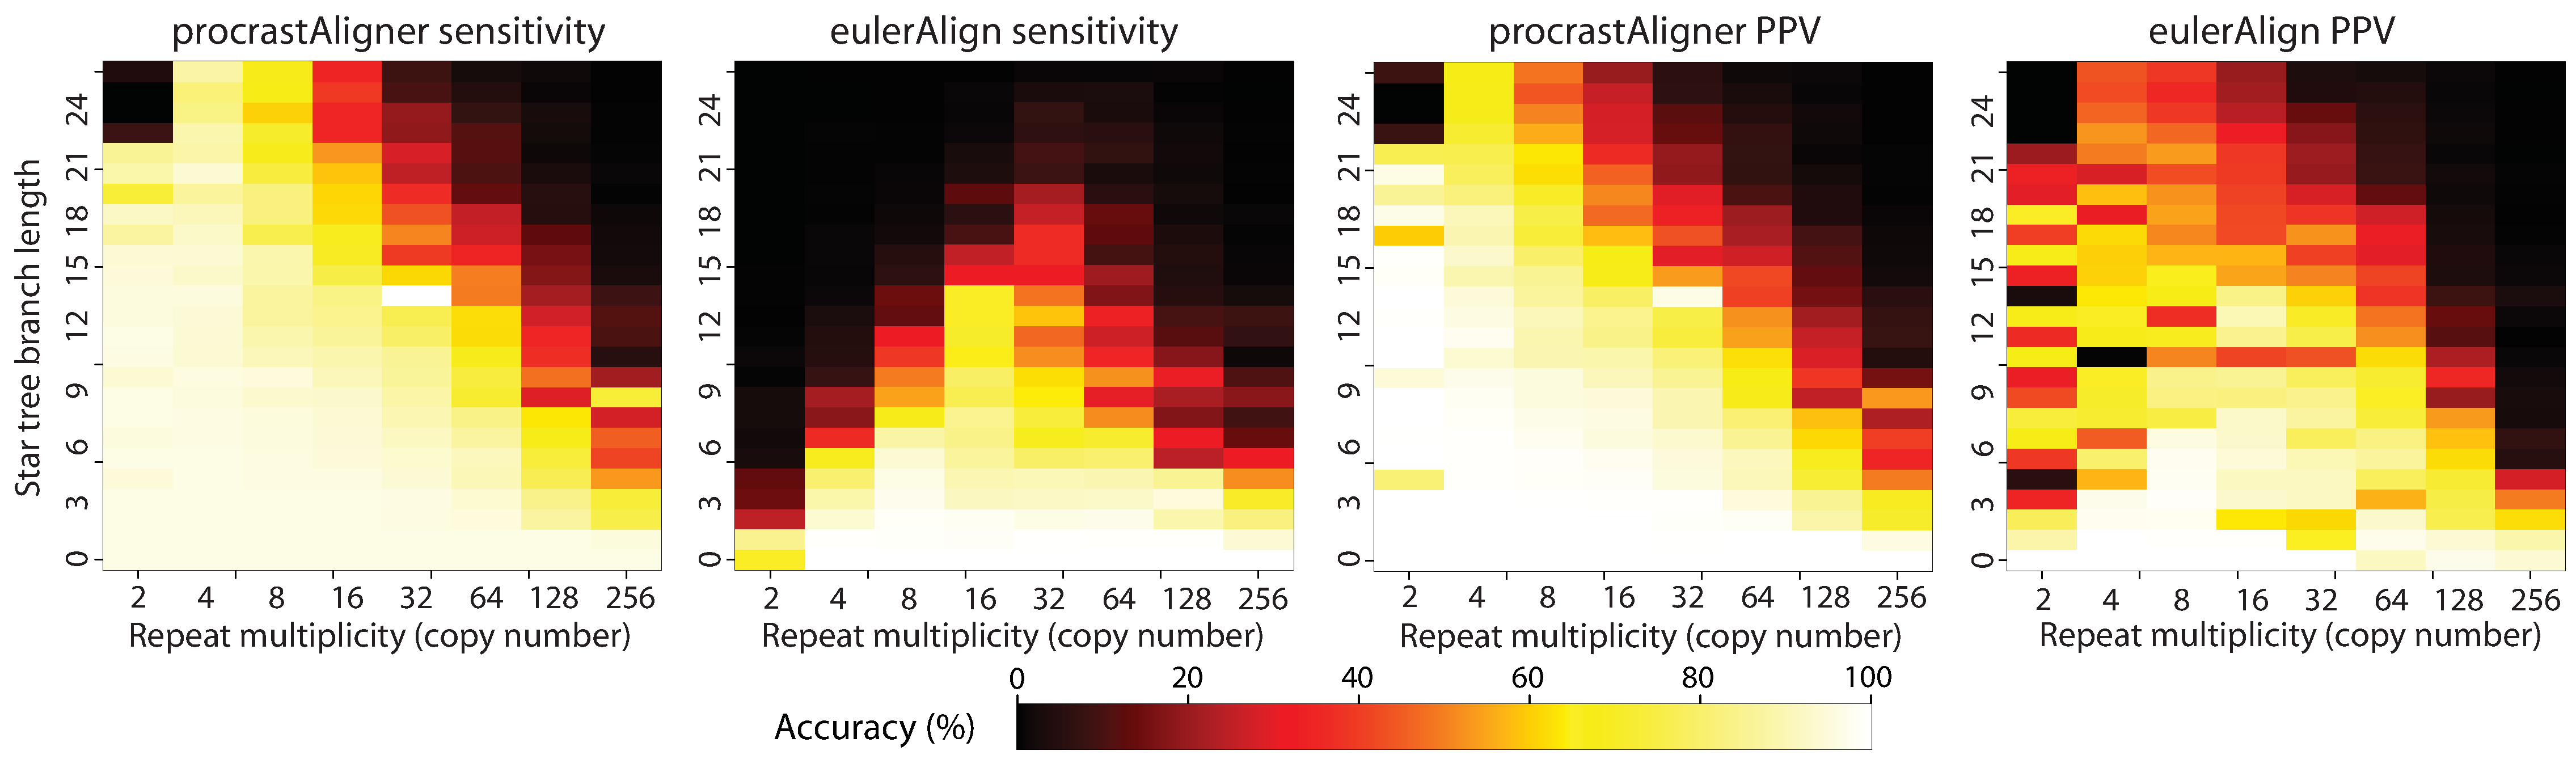
\epsfig{file=./fig/repeat_accuracy_new.eps,width=6.8in}
\caption[Accuracy recovering simulated repeat families planted in the
\textit{Mycoplasma genitalium} genome]%
{\textbf{Accuracy recovering simulated repeat families planted in the
\textit{Mycoplasma genitalium} genome}.  Sum-of-pairs nucleotide
sensitivity and positive predictive value (PPV) of \texttt{procrastAligner}
and \texttt{eulerAlign} were measured for 200
combinations of branch length and multiplicity.  Three replicates of
each simulation were performed and average accuracy values are shown
here.  White points indicate perfect alignment of the simulated repeat
family.  Black points indicate the program completely failed to
recover any portion of the repeat family.  Average mutations per site can be
calculated by multiplying branch length by the fixed substitution rate
of 0.09, and indel rate of 0.01.  For example, at branch length 20
there are 1.8 substitutions per site and 0.2 indels per site.  From
the figure, it is apparent that \texttt{procrastAligner} performs better
at higher mutation rates and multiplicities than \texttt{eulerAlign}.}
\label{fig-results}
\end{figure*}
\subsection{Adapting HMM parameters from an arbitrary substitution matrix to organisms with different G+C content}
HMM probabilities can be derived using any strand/species symmetric nucleotide substitution matrix,
but any particular matrix makes specific assumptions about divergence time, mutation pressures,
and sequence composition of the aligned sequences.
Genomes can range in G+C content from 30-75\%, and at the extremes,
a substitution matrix derived on 47.5\% GC sequence (such as HOXD70) does not
perform well.  We have thus developed a method to adapt HMM emission
probabilities derived from an arbitrary substitution matrix
to organisms with different G+C content.

Emission
probabilities in the Unrelated state can be directly adapted to the
background nucleotide distribution as follows:
\begin{multline}\\
U_{AA}=U_{AT}=U_{TA}=U_{TT}=(\frac{f_{AT}}{2})(\frac{f_{AT}}{2})\\
U_{CC}=U_{CG}=U_{GC}=U_{GG}=(\frac{f_{GC}}{2})(\frac{f_{GC}}{2})\\
U_{AC}=U_{AG}=U_{TC}=U_{AG}=(\frac{f_{AT}}{2})(\frac{f_{GC}}{2})\\
U_{CA}=U_{CT}=U_{GA}=U_{GT}=(\frac{f_{GC}}{2})(\frac{f_{AT}}{2})\\
\end{multline}
where the notation $U_{XY}$ indicates the probability of observing nucleotide X aligned to
nucleotide Y in Unrelated sequence.  $f_{AT}$ is the fraction of nucleotides which are A/T and
$f_{GC}$ is the fraction of G/C in the input genome.  Note that $f_{AT}=1-f_{GC}$.

To adapt emission probabilities in the homologous state, we consider the
probability of nucleotide substitution under the standard assumption
that sequences evolve according to a continuous-time reversible Markov process.
Thus, the probability of nucleotide $X$ mutating to nucleotide $Y$ over time $t$
can be written as: $H_{XY}=\pi_X Q(X,Y)t$, where $\pi_X$ represents the background
frequency of nucleotide $X$ and $Q(X,Y)$ is the instantaneous substitution rate for $X$
mutating to $Y$. Because the background frequencies on which the substitution matrix was computed are
known (e.g. 47.5\%GC for HOXD70), we can simply replace the $\pi_X$ from the HOXD70 matrix
with the $\pi'_X$ from the input genome. Given that the substitution process is
strand-symmetric and reversible, we can compute adapted
emission probabilities for the Homologous state as follows:
\begin{multline}\\
H'_{AG}=H_{AG}\\
H'_{AC}=H_{AC}\\
H'_{AA}=(\frac{f'_{AT}}{f_{AT}})H_{AA}\\
H'_{AT}=(\frac{f'_{AT}}{f_{AT}})H_{AT}\\
H'_{CC}=(\frac{f'_{GC}}{f_{GC}})H_{CC}\\
H'_{CG}=(\frac{f'_{GC}}{f_{GC}})H_{CG}\\
\end{multline}
where $f'_{AT}$ and $f'_{GC}$ represent the input genome's AT and GC content,
$H_{XY}$ values are the original emission probabilities derived from the
substitution matrix, and $H'_{XY}$ are emission probabilities adapted to
the input genome's G+C content.

%\section{Configuring the transition probabilities of the HMM}


\section{Calculating the posterior probability of alignment columns}
Using the empirically derived transition and emission probabilities,
we apply the posterior HMM decoder implemented in Gerton Lunter's
HMMoC software~\cite{Lunter2007} to compute the posterior probability (p.p.) that
each alignment column represents homologous sequence.  Columns with a
p.p. below 0.5 are considered to be unrelated; use of 0.5 as a p.p. threshold
yields a maximum \textit{a posteriori} estimate of homology.  We then apply the
transitive homology principle to our predictions, resulting in a final
set of consistent homology predictions.  See Figure~\ref{fig-main},
steps 5 and 6 for an example. We trim the alignment to exclude all
columns beyond the Homologous state. If the original boundaries were
improved, we trigger another round of chaining (and consequently
another round of extension) in the same direction.
When gapped extension fails to improve boundaries
in one direction, extension in the other direction is attempted until
no further extension is possible.

\begin{figure*}[t!]
\centering
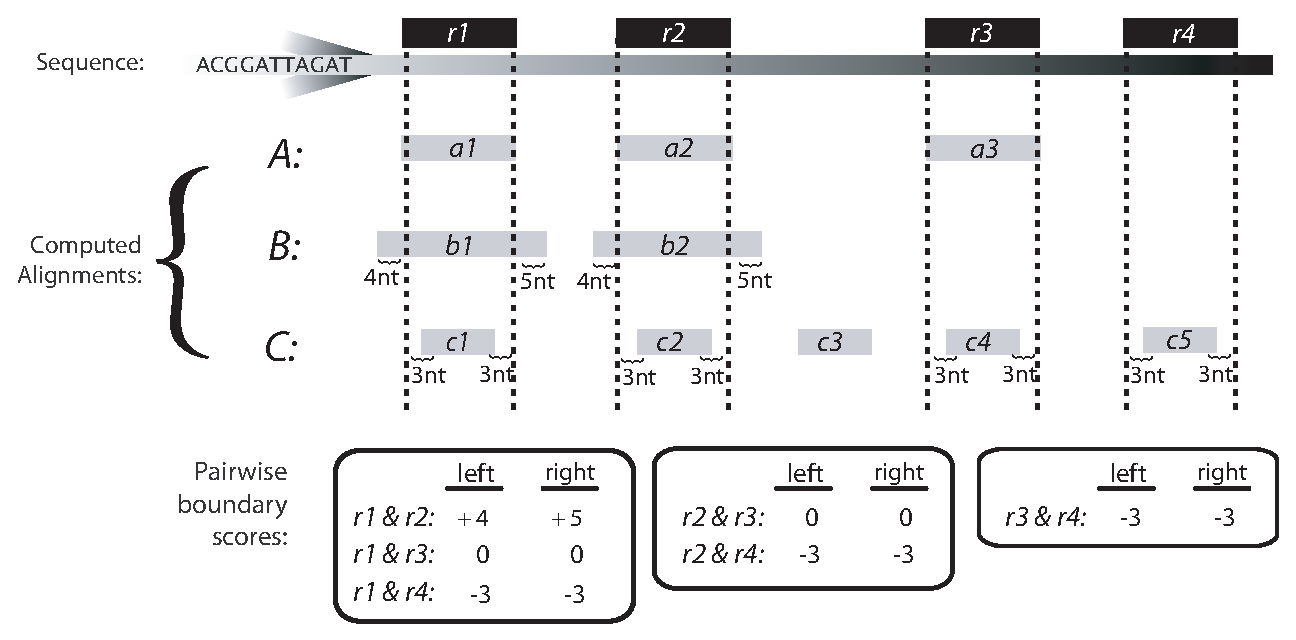
\epsfig{file=./fig/boundary_scores.eps,width=6.5in}
\caption[Pairwise boundary accuracy metric]%
{\textbf{Pairwise boundary accuracy metric}. We define our boundary accuracy metric to be an all-pairs score by comparing the boundaries of all \emph{r} components of the inserted repeat \emph{R} to the boundaries predicted by the alignment program. For any pair of components, $\emph{r}_{i}$ and $\emph{r}_{j}$, we take the maximum boundary of any local multiple alignments output by the program. The figure shows a multiplicity five interspersed repeat \emph{R} and four local multiple alignments, \emph{A, B, C, D}.  Boundary predictions can be classified as (1) correct, (2) overprediction, and (3) underprediction, with each discussed in turn: (1) \emph{Correct prediction}. Consider scoring components \emph{r1} and \emph{r3}.  Local multiple alignment \emph{A} overlaps both \emph{r1} and \emph{r3} and no other alignment overlaps both \emph{r1} and \emph{r3}.  The left and right boundaries of alignment \emph{A} match the boundaries of \emph{r1\&r3} exactly, thus we assign scores of 0 for \emph{r1\&r3}.  (2) \emph{Overprediction}. Consider scoring components \emph{r1} and \emph{r2}.  These components are overlapped by alignments \emph{A} and \emph{C}.  Alignment \emph{A} has perfect boundary predictions for \emph{r1\&r2}, while alignment \emph{C} extends beyond the true boundaries of components \emph{r1} and \emph{r2} by 4 nucleotides on the left and 5 nucleotides on the right.  Our scoring metric always uses the maximum predicted boundaries for a pair of components, thus the boundary predictions from \emph{C} are reported for \emph{r1\&r2}. (3) \emph{Underprediction.}  Consider scoring components \emph{r3} and \emph{r5}.  Alignment \emph{B} hits both \emph{r3} and \emph{r5}, but stops short of the right-side boundary by 8nt in \emph{r3} and 4nt in \emph{r5}.  We average the error and record -6 for the right-side of \emph{r3\&r5}.
Finally, component pairs that are not contained by any computed alignments are not scored, as indicated by \emph{n/a}.}
\label{fig-overunder}
\end{figure*}
\section{Results}
We have previously demonstrated the sensitivity of our chaining method
in finding Alu repeats in the human
genome~\cite{ref-procrast}. Figure~\ref{fig-align} shows part of a
local multiple alignment of one such Alu family as generated with
\texttt{procrastAligner}. To highlight the benefits of our proposed
heuristic for gapped extension, we compare ~\texttt{procrastAligner}'s
performance to the Eulerian path method for local multiple alignment
as implemented by \texttt{eulerAlign}~\cite{ref-related1}. The Eulerian
path method uses a \textit{de Bruijn} graph for filtration, and goes
beyond filtration to compute gapped alignments using banded dynamic
programming.  To our knowledge, \texttt{procrastAligner} and
\texttt{eulerAlign} represent the only two automated methods to
construct local multiple alignments directly from genomic DNA.

\subsection{Simulating interspersed repeats}
We evaluate accuracy of each method when aligning simulated repeat
families that have been inserted into the complete genome of
\emph{Mycoplasma genitalium}. The \emph{M. genitalium} genome has been recognized
as complex and repeat-rich, presenting a biologically
relevant and challenging example to evaluate alignment
methods~\cite{ref-mycoplasma}. We simulated repeat families of 8
different multiplicities ranging between 2 and 256 ($x$-axis in
Figure~\ref{fig-results}).  Each repeat copy has an average length
based on its family's multiplicity
($length=\frac{7680}{multiplicity}$), thus high copy-number repeats
are short.  Evolution of repeat families was simulated as a marked
Poisson process on a star tree
topology.  The branch lengths were varied between 0 and 24 ($y$-axis
in Figure~\ref{fig-results}), with the nucleotide substitution rate
fixed at 0.09 per unit time, and the indel rate fixed at 0.01 per
unit time.  Rate heterogeneity among sites was modeled with a gamma
distribution ($\theta = 1.0, k = 0.5$).  Indel size was
Poisson distributed with intensity 3, and insertions and deletions
were taken to be equally likely.  Each family's ancestral
sequence was randomly generated using nucleotide frequencies equal to
the composition of \emph{Mycoplasma genitalium}
($A=0.34,T=0.34,G=0.16,C=0.16$). Insertion sites for repeat copies
were chosen uniformly at random in the 580kb \textit{M. genitalium} genome,
allowing tandem repeats but prohibiting mosaic repeats.
\begin{figure*}[ht!]
\centering
\subfigure[]{
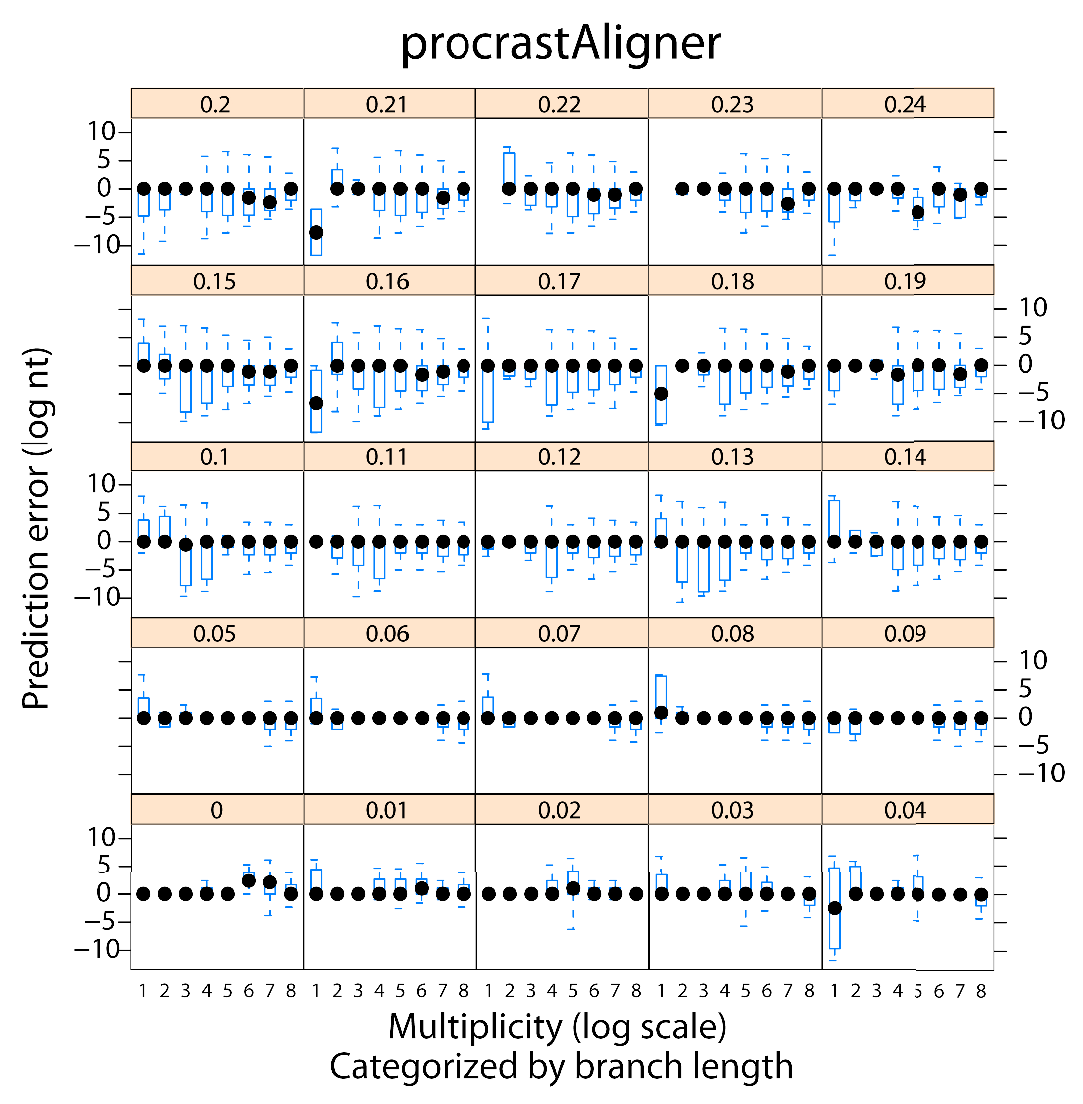
\epsfig{file=./fig/procrast_boundary_fig.eps,width=3.3in}
\label{fig:subfig1}}
\subfigure[]{
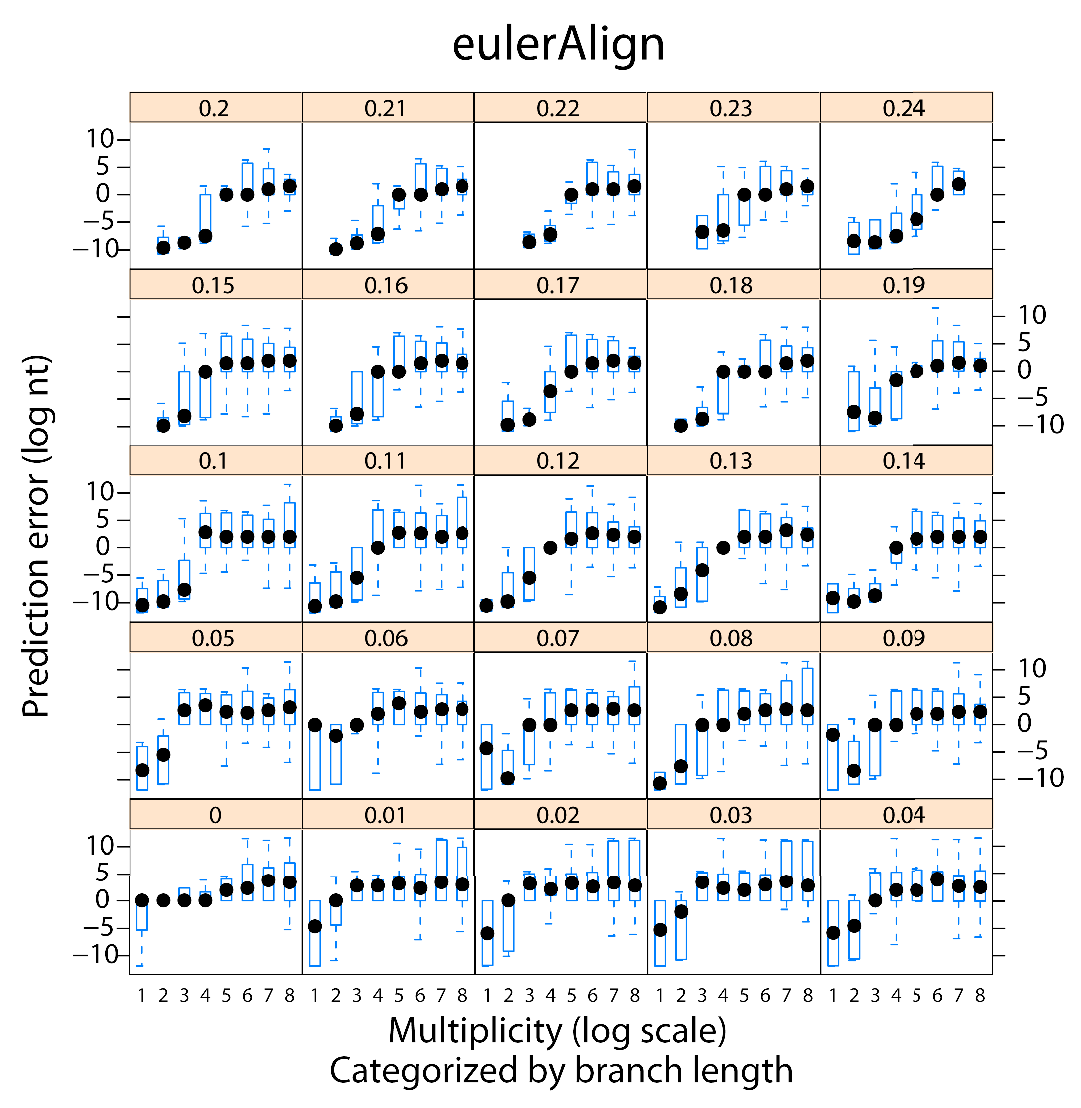
\epsfig{file=./fig/euler_boundary_fig.eps,width=3.3in}
\label{fig:subfig2}}
\caption[Boundary prediction performance]%
{\textbf{Boundary prediction performance}. All-pairs boundary prediction accuracy of \texttt{procrastAligner} and \texttt{eulerAlign} were measured for 200 combinations of branch length and multiplicity.  Accuracy on each combination is presented as a box-and-whiskers plot using the scoring metric detailed in Section~\ref{sec:metrics}.  Branch lengths range from 0 to 0.24 and increase by intervals of 0.01.  The $x$-axis label represents the multiplicity of the interspersed repeat in log$_2$-scale. i.e. axis label 8 indicates $2^{8}$ = multiplicity 256. The $y$-axis label is the prediction error in log$_2$-scale nucleotides. Values at 0 represent correctly identified repeat boundaries, values greater than 0 represent overpredictions, and values less than 0 represent underpredictions (see Figure~\ref{fig-overunder}). In general, \texttt{procrastAligner} identifies the true interspersed repeat boundaries more accurately than \texttt{eulerAlign}.}
\label{fig-boundary}
\end{figure*}
\subsection{Alignment accuracy metrics}
\label{sec:metrics}
We used each program to find local multiple alignments in each of the
200 modified \emph{M. genitalium} genomes and recorded alignment
accuracy as follows. We calculated sum-of-pairs nucleotide sensitivity
as $\frac{\mathrm{TP}}{\mathrm{TP} + \mathrm{FN}}$, where
$\mathrm{TP}$ is the number of aligned nucleotide pairs in the
program's output which are also aligned in the simulated repeat
family.  $\mathrm{FN}$ is the number of aligned nucleotide pairs in
the simulated repeat family which are missing from the program's
output.  This sensitivity measure is identical to the sum-of-pairs
accuracy defined by BaliBASE~\cite{ref-balibase}.  We calculate the
positive predictive value (PPV) as $\frac{\mathrm{TP}}{\mathrm{TP} +
\mathrm{FP}}$, where $\mathrm{TP}$ is defined as above, and
$\mathrm{FP}$ is the total number of nucleotide pairs from the
program's output where one of the nucleotides are part of the
simulated repeat family and the other nucleotide was incorrectly
aligned. We also quantify the ability of each aligner to accurately predict the
boundaries of the interspersed repeats.  For a given pair of repeat components, we calculate accuracy by recording the number of nucleotides between the true boundary and the predicted boundary
on both the right and left sides of the repeat.  Thus, over-extension gets a positive score, while underextension
yields a negative score and perfect boundaries receive a 0 score. See Figure~\ref{fig-overunder} for
further details on boundary under/overpredictions.


\subsection{Accuracy when aligning interspersed repeats}
We applied \texttt{procrastAligner} and \texttt{eulerAlign} to the
hybrid simulated/real dataset.  We ran \texttt{procrastAligner}
with command-line parameters \texttt{--z=15 --w=20}, and
\texttt{eulerAlign} with \texttt{-k 15 -l -i 1000 -v} based on suggestions
from the program's user guide and manual experimentation.
Simulations for each of the 200 combinations of branch length and
multiplicity were replicated three times and alignments generated in
parallel on a 156-node compute cluster.  Also, we adapted the default \texttt{procrastAligner} HMM emission probabilities based on HOXD70 to 95\% sequence identity (\texttt{--percentid=0.95}), since the default 65-70\% identity would be too low for the majority of mutation rates.  Results of the experiments
are reported in Figure~\ref{fig-results} and
Figure~\ref{fig-boundary}. Figure~\ref{fig-results} illustrates the
sensitivity and PPV of
\texttt{procrastAligner} and
\texttt{eulerAlign} on datasets ranging from 0 substitutions and
indels per site to 2.16 substitutions and 0.24 indels per site (branch length 24).  As
mutation rates and repeat multiplicity increase the alignment accuracy
decreases for both methods, with accuracy of \texttt{eulerAlign}
decreasing faster than \texttt{procrastAligner}.  Surprisingly, \texttt{eulerAlign}
often fails to align low multiplicity repeats, even when mutation rates are low.
Manual experimentation with \texttt{eulerAligner} parameters, such as: -v (tolerance for mismatches), -k (seed $k$-mer size) from 11 to 15, and -i (number of iterations) from 1000 up to 10,000, failed to improve its performance on low-multiplicity repeats.
We conjecture that \texttt{procrastAligner}'s overall improved accuracy largely derives
from its use of spaced seed patterns~\cite{ref-procrast} and tolerance
of gaps. With the \texttt{-v} option enabled, the Eulerian path method allows up to 10\% mismatches for matching $k$-mers to seed gapped alignment extensions. While this certainly improves the sensitivity at lower mutation rates, the experimental results presented Figure~\ref{fig-results} show that it is inadequate for higher mutation rates.In addition to sensitivity and PPV benchmarks, we also assess how well
each aligner recovers the true boundaries of interspersed
repeats.  Figure~\ref{fig-boundary} illustrates the ability of each
program to accurately localize the known boundaries of the simulated interspersed
repeats. From the figure, it is apparent that on average, \texttt{procrastAligner} predicts
the exact repeat boundary for all studied combinations of branch length (repeat degeneracy)
and multiplicity (repeat copy number).  Moreover, the standard error in \texttt{procrastAligner}'s
boundary predictions is typically very low, within 4 nucleotides.  \texttt{eulerAlign}, on the other hand,
exhibits more erratic behavior.  For low multiplicity repeats it has a strong tendency to
underpredict the repeat boundary.  At high multiplicities ($\geq32$) \texttt{eulerAlign} tends to
slightly overpredict the boundaries, by including flanking unrelated sequence in the alignment of
the interspersed repeat.  And as expected, when using the default \texttt{procrastAligner} HMM emission probabilities resulted in no underpredictions, although the overpredictions were more abundant (data not shown).
%\subsection{Runtime comparison}

Finally, a direct comparison of run time is difficult, due to the differing natures of the local multiple alignment programs.  \texttt{eulerAlign} runtime depends on the iterations parameter, which controls the total number of local multiple alignments reported, whereas \texttt{procrastAligner} reports \textit{all} local multiple alignments in a single run.  Despite this, we report the average per-experiment CPU time for each program on the test dataset. \texttt{procrastAligner} required on average 55 seconds per experiment, with the longest taking just over two minutes. \texttt{eulerAlign} required 1 hour total compute time per experiment on average, which equates to about 4 seconds per iteration.  Both programs exhibited similar memory usage, \texttt{procrastAligner} requiring on average 50 MB per experiment and \texttt{eulerAlign} requiring on average 70 MB per experiment.

\begin{figure*}[ht!]
\centering 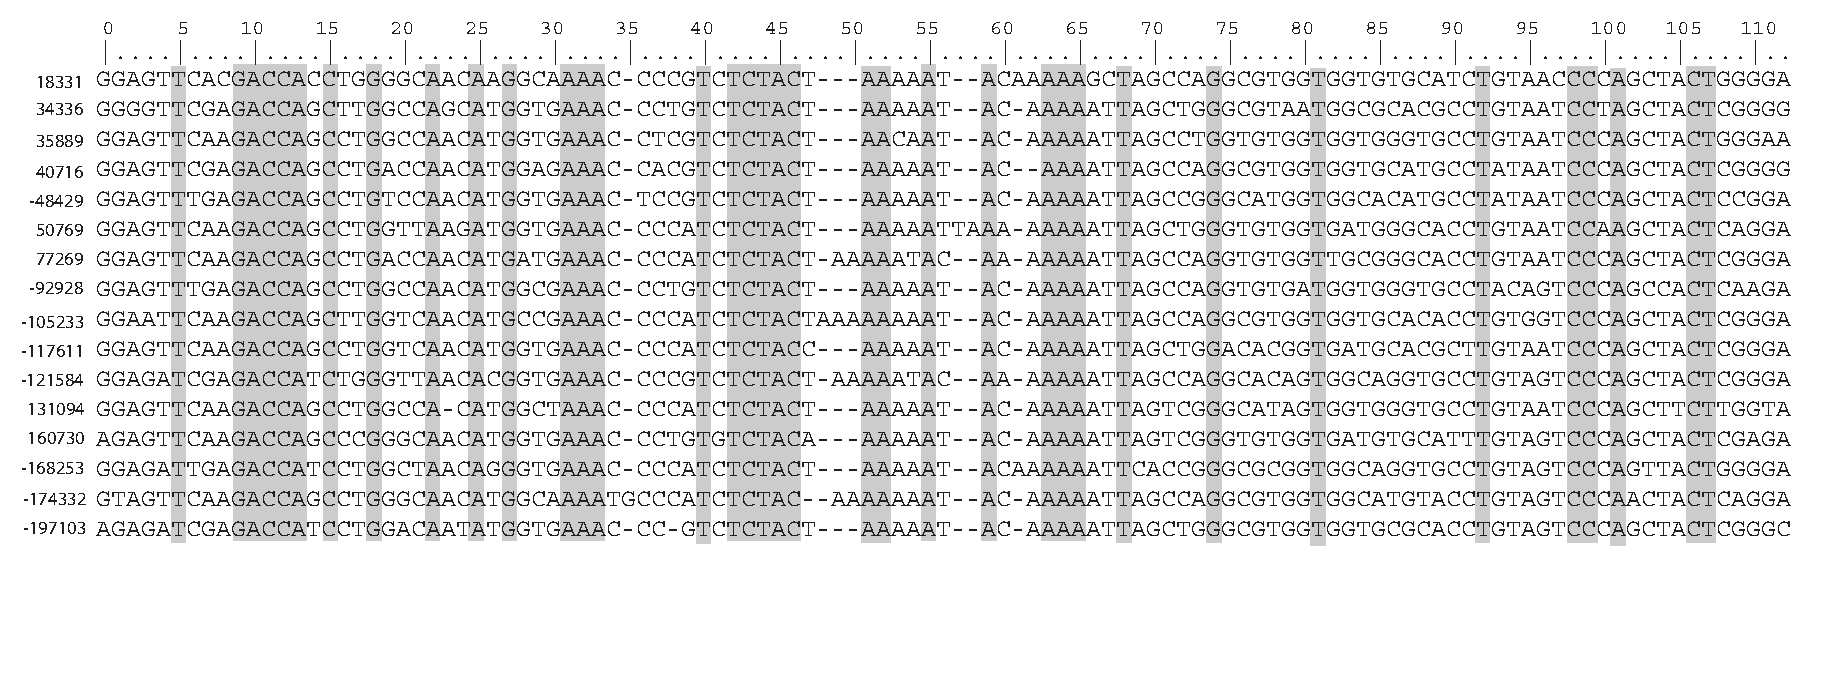
\epsfig{file=./fig/alu_align.eps,width=6.8in}
\vspace{-1.0cm}
\caption[Alu repeat alignment]%
{\textbf{Alu repeat alignment}. Partial view of an Alu repeat alignment output by procrastAligner in the \emph{H. sapiens} BAC
clone RP11-355H10 (Accession AC010145.10). Each row represents an
aligned Alu. Highlighted columns indicate conserved sequence among all
16 copies of the Alu. Start positions are shown to the left, negative
values indicate complement strand.  Local multiple alignment was
generated with \texttt{procrastAligner} with parameters: \texttt{--z=9
--w=50}.  }
\label{fig-align}
\end{figure*}
\section{Estimating significance of local multiple alignments}
Increased seed matching sensitivity creates additional
false positive seed hits, so a statistical test for rejecting
insignificant local alignments is essential.  BLAST statistics have proven
invaluable for assessing the significance of pairwise local alignments, for amino acid and nucleotide sequences.
Fast methods to approximate the significance of pairwise
repeats have been implemented~\cite{repseek} and potentially can be
extended to multiple alignments~\cite{ref-related1, Prakash2005}.  We
now describe the method we use for estimating significance of local
multiple alignments.

For the present work, we are concerned not with random similarity between two or more sequences, but rather, random similarity arising within a single sequence.  We would like to compute the likelihood that a given repeat would appear by chance in order to decide whether the repeat reflects true sequence homology or random similarity.  Much effort has been expended to derive the probability of finding a segment of score $S$ between two sequences (see~\cite{Ewens2001} and references therein) or shared by $k$ sequences~\cite{ref-related1}. These statistics~\cite{Karlin1990} show that, $N$, the number of high scoring similarity segments between two sequences of size $m$ and $n$ with a score $S \geq x$ converges to:

\begin{equation}
    E[ N_{(S\geq x)} ] = Kmn p^x
    \label{E_mn}
\end{equation}

$K$ is a scale parameter that depends on the scoring system and $p$ (also often seen as $p=e^{-\lambda}$) can be understood as the per site probability of finding a segment of score 1. Using a Poisson approximation, the probability that the largest score is greater than or equal to $x$ is given by:

\begin{equation}
    P( S_1 \geq x) = 1 - exp( -E[ N_{(S\geq x)} ] )
    \label{P_s1}
\end{equation}

For gap-free alignments, both parameters $K$ and $p$ can be computed numerically~\cite{Karlin1990} whereas their estimation relies on simulations when gaps are allowed  ~\cite{Waterman1994, Altschul2001}.

The above statistics to compute expectation of matching across two sequences can be easily extended to 2-copy repeats within the same strand of a sequence of size $n$, by substituting $mn$ by ${{n}\choose{2}}$ in the above equations. Taking both strands of DNA into account, we have to count successively cases where 0,1 or 2 copies are on the forward strand; copies on the same strand can be swapped without changing the repeat structure. Because of the symmetry, the number of possible positions is halved. Therefore, the expected number of 2-copy repeats on both strands with a score greater or equal than $x$ is:

\begin{eqnarray}
    E[ N_{(r=2, S\geq x)} ]  & = & K \times  \Big( n (n-1) \frac 12 (\frac 1 2 + 1 + \frac 1 2) \Big) \times  p^x \nonumber \\
                                          & = & K  n (n-1)   p^x
    \label{E_r2}
\end{eqnarray}


More generally, the expected number of repeats of multiplicity $r$ on both strands that have a score greater than or equal to $x$ is given by:

\begin{equation}
    E[ N_{(r, S\geq x)} ]   =  K \times  \Big( \frac{n!}{(n-r)! }  \frac 12 \sum_{k=0}^{r}{\frac{1}{k! (r-k)!}} \Big) \times  p^{(r-1)x}
    \label{E_repeat}
\end{equation}

In the above equation, the two unknown parameters $K$ and $p$ can be estimated on 2-copy repeats using random sequences of the same size and identical composition.  This can be done by using either the direct method~\cite{Olsen1999} with a $log(-log(1-P))$ transformation of the Equation \ref{P_s1}, or by using the declumping method ~\cite{Waterman1994}, or by the island method~\cite{Olsen1999} using a $log(E)$ of Equation \ref{E_r2}. Once $K$ and $p$ are estimated, Equation \ref{P_s1} along with Equation \ref{E_repeat} can be used to asses the probability of any observed repeat of a given score and a given multiplicity. An adequate score to be used is the average pairwise alignment score of repeat components.  

%Importantly, these equations show a perfect fit with repeats from random genomes (data not shown).

Although our significance measure for local multiple alignments is only an approximation, its introduction will allow
for increased sensitivity (i.e. smaller seed size, seed families) while maintaining specificity. The statistical
test helps to filter out spurious alignments, although it doesn't resolve redundant alignments. To address redundant alignments, we follow
the approached proposed in~\cite{ref-related1} by grouping all alignments which share at least one aligned column. Then, we can select the reference alignment
as the alignment in the group with the highest Sum-of-Pairs (SP) score, breaking ties either by multiplicity or repeat length. The selection of a reference alignment from each redundant group can be defined by the user via a command-line parameter, allowing for the reference alignment to be tailored towards specific repeat analysis tasks.



\section{Conclusion}
We have presented a sensitive and efficient gapped-extension heuristic for local
multiple alignment. We have extended our previous results by
converting chains of ungapped multi-matches into gapped local multiple
alignments. We have also added a method to remove spurious local multiple alignments by introducing a statistical estimation of significance
performed directly on the input sequence.  Experimental results demonstrate that the
described method offers a level of alignment accuracy exceeding
that of a related method. Accurately predicting homology boundaries has important implications; for example, tools to build repeat family databases can directly use the alignments without the manual curation required in current approaches and also is likely to aid in the evolutionary analysis of transposon proliferation.  With respect to the boundary prediction accuracy, we would like to emphasize the importance of correctly selecting an appropriate substitution matrix for the expected amount of divergency among the repeats. The default subsitution matrix our program uses is the HOXD70 matrix, which is optimized for 70\% sequence identity. Thus, using the default substitution matrix when performing repeat detection on less diverged families can result in overextended repeat boundaries, or vice versa.

Further improvement of the alignment methodology will likely require increasingly sensitive methods for
seed matching. One possible avenue to increase seed matching sensitivity and reduce boundary underpredictions would be merging overlapping seed matches into a
shorter, higher-multiplicity match.  A second avenue would be to use palindromic seed families instead of using a single seed pattern~\cite{ref-pattern}.

\subsection{Implementation}
We have implemented our method in a program, \texttt{procrastAligner},
available for Linux, Windows, and Mac OS X. Our open-source
implementation is available as C++ source code licensed under the GPL , and can be downloaded from:
\url{http://alggen.lsi.upc.es/recerca/align/procrastination}.

\section{ Acknowledgment }
The authors would like to thank Yu Zhang for providing the
\texttt{eulerAlign} program. We would also like to thank
Webb Miller for providing the HOXD70 substitution matrix data. Accuracy
evaluations utilized a compute resource grant from the Australian
Partnership for Advanced Computing.  AED was supported by NSF grant
DBI-0630765. TJT was supported by Spanish Ministry MECD Grant
TIN2004-03382 and AGAUR Training Grant FI-IQUC-2005.

% trigger a \newpage just before the given reference
% number - used to balance the columns on the last page
% adjust value as needed - may need to be readjusted if
% the document is modified later
%\IEEEtriggeratref{8}
% The "triggered" command can be changed if desired:
%\IEEEtriggercmd{\enlargethispage{-5in}}

% references section
% NOTE: BibTeX documentation can be easily obtained at:
% http://www.ctan.org/tex-archive/biblio/bibtex/contrib/doc/

% can use a bibliography generated by BibTeX as a .bbl file
% standard IEEE bibliography style from:
% http://www.ctan.org/tex-archive/macros/latex/contrib/supported/IEEEtran/
%\bibliographystyle{IEEEtran.bst}
% argument is your BibTeX string definitions and bibliography database(s)
%\bibliography{IEEEabrv,../bib/paper}
%
% <OR> manually copy in the resultant .bbl file
% set second argument of \begin to the number of references
% (used to reserve space for the reference number labels box)

\bibliographystyle{IEEEtran}
\bibliography{procrastination}
%%\documentclass[draft]{ws-procs9x6}
\documentclass{llncs}
\usepackage{color}
\usepackage{epsfig}
\usepackage{times}
\usepackage{url}
\begin{document}
\chapter*{Supplementary Material}
\section*{Calculating the Chiaromonte \textit{et al.} scaling factor}
The emission probabilities for
each possible pair of aligned nucleotides were extracted from the HOXD
substitution matrix presented by Chiaromonte \textit{et al}\cite{hoxd}.
We solved for the emission frequencies in the
Homologous and Unrelated state using the same equation used to
calculate the values of the HOXD substitution matrix on 47.5\%G+C
content sequence\cite{hoxd}:
\begin{equation}
s(x,y)= \log_{2}{\Bigg(\frac{p(x,y)}{q_{1}(x)q_{2}(y)}\Bigg)}
\end{equation}
{w}here $p(x,y)$ is the fraction of the observed aligned pairs of
nucleotides $x$ and $y$ in the training set used and $q_{1}(x)$ and
$q_{2}(x)$ denote the background frequencies of $x$ and $y$,
respectively. Chiaramonte \textit{et al.} scaled the resulting
$s(x,y)$ values by an unreported value $\psi$ so the largest was 100,
with the rest rounded to the nearest integer.  Given that the training
data has $47.5\%$~$G+C$ content and considering strand and species
symmetry, we can compute emission frequencies for the Unrelated state
of our HMM:
\begin{center}$U_{AA}=U_{AT}=U_{TA}=U_{TT}=(\frac{f_{AT}}{2})(\frac{f_{AT}}{2})
= 0.06890625$ \\
$U_{CC}=U_{CG}=U_{GC}=U_{GG}=(\frac{f_{GC}}{2})(\frac{f_{GC}}{2}) =
0.05640625$ \\
$U_{AC}=U_{AG}=U_{TC}=U_{AG}=(\frac{f_{AT}}{2})(\frac{f_{GC}}{2}) =
0.06234375$ \\
$U_{CA}=U_{CT}=U_{GA}=U_{GT}=(\frac{f_{GC}}{2})(\frac{f_{AT}}{2}) =
0.06234375$ \\
\end{center}

Where $f_{GC}=0.475$ and $f_{AT}=0.525$ are background frequencies of
G/C and A/T, respectively.  Then we derive emission probabilities for
the Homologous state as, for example:
\begin{equation}
\log_{2}\bigg(\frac{H_{AA}}{U_{AA}}\bigg) = \frac{91}{\psi},
\end{equation}
where $\frac{1}{\psi}$ is the unknown scaling factor used normalize $H_{CC}$ to 100. The full list of equations follows:
\begin{center}
$\log_{2}\bigg(\frac{H_{AC}}{U_{AC}}\bigg) = \frac{-114}{\psi},$
$\log_{2}\bigg(\frac{H_{AG}}{U_{AC}}\bigg) = \frac{-31}{\psi}$ \\
$\log_{2}\bigg(\frac{H_{AT}}{U_{AC}}\bigg) = \frac{-123}{\psi},$
$\log_{2}\bigg(\frac{H_{CG}}{U_{CC}}\bigg) = \frac{-125}{\psi}$ \\
$\log_{2}\bigg(\frac{H_{AA}}{U_{AA}}\bigg) = \ \ \ \frac{91}{\psi},$
$\log_{2}\bigg(\frac{H_{CC}}{U_{CC}}\bigg) = \ \ \ \frac{100}{\psi}$ \\
\end{center}

The system of six equations has seven free variables.  Moreover, the $H_{xy}$ must sum to 1 to make a probability distribution:
\begin{equation}
H_{AA} + H_{AC} + H_{AG} + H_{AT} + H_{CC} + H_{CG} = 1
\end{equation}
%$0.03072937146$
%$32.54215601$
We can solve the above six equations for $H_{xy}$ and substitute the
resulting expressions in to the normalizing equation to solve for
$\psi$. For the HOXD matrix the scaling factor is $\psi=32.5421$. Given
$\psi$, we can calculate values for all $H_{xy}$.

\bibliographystyle{splncs}
\bibliography{procrastination}
\end{document}




% You can push biographies down or up by placing
% a \vfill before or after them. The appropriate
% use of \vfill depends on what kind of text is
% on the last page and whether or not the columns
% are being equalized.

%\vfill

% Can be used to pull up biographies so that the bottom of the last one
% is flush with the other column.
%\enlargethispage{-5in}

% that's all folks
\end{document}
